% do not change these two lines (this is a hard requirement
% there is one exception: you might replace oneside by twoside in case you deliver 
% the printed version in the accordant format
\documentclass[11pt,titlepage,oneside,openany]{book}
\usepackage{times}


\usepackage{graphicx}
\usepackage{caption}
\usepackage{subcaption}
\usepackage{url}
\usepackage{hyperref}
\usepackage{latexsym}
\usepackage{amsmath}
\usepackage{amssymb}
\usepackage{booktabs}
\usepackage{multirow}
\usepackage{makecell}
\usepackage{tablefootnote}
\usepackage{outlines}

\usepackage{ntheorem}

% \usepackage{paralist}
\usepackage{tabularx}

% this packaes are useful for nice algorithms
\usepackage{algorithm}
\usepackage{algorithmic}

% well, when your work is concerned with definitions, proposition and so on, we suggest this
% feel free to add Corrolary, Theorem or whatever you need
\newtheorem{definition}{Definition}
\newtheorem{proposition}{Proposition}


% its always useful to have some shortcuts (some are specific for algorithms
% if you do not like your formating you can change it here (instead of scanning through the whole text)
\renewcommand{\algorithmiccomment}[1]{\ensuremath{\rhd} \textit{#1}}
\def\MYCALL#1#2{{\small\textsc{#1}}(\textup{#2})}
\def\MYSET#1{\scshape{#1}}
\def\MYAND{\textbf{ and }}
\def\MYOR{\textbf{ or }}
\def\MYNOT{\textbf{ not }}
\def\MYTHROW{\textbf{ throw }}
\def\MYBREAK{\textbf{break }}
\def\MYEXCEPT#1{\scshape{#1}}
\def\MYTO{\textbf{ to }}
\def\MYNIL{\textsc{Nil}}
\def\MYUNKNOWN{ unknown }
% simple stuff (not all of this is used in this examples thesis
\def\INT{{\mathcal I}} % interpretation
\def\ONT{{\mathcal O}} % ontology
\def\SEM{{\mathcal S}} % alignment semantic
\def\ALI{{\mathcal A}} % alignment
\def\USE{{\mathcal U}} % set of unsatisfiable entities
\def\CON{{\mathcal C}} % conflict set
\def\DIA{\Delta} % diagnosis
% mups and mips
\def\MUP{{\mathcal M}} % ontology
\def\MIP{{\mathcal M}} % ontology
% distributed and local entities
\newcommand{\cc}[2]{\mathit{#1}\hspace{-1pt} \# \hspace{-1pt} \mathit{#2}}
\newcommand{\cx}[1]{\mathit{#1}}
% complex stuff
\def\MER#1#2#3#4{#1 \cup_{#3}^{#2} #4} % merged ontology
\def\MUPALL#1#2#3#4#5{\textit{MUPS}_{#1}\left(#2, #3, #4, #5\right)} % the set of all mups for some concept
\def\MIPALL#1#2{\textit{MIPS}_{#1}\left(#2\right)} % the set of all mips

\DeclareMathOperator*{\argmax}{arg\,max}
\DeclareMathOperator*{\argmin}{arg\,min}





\begin{document}

\pagenumbering{roman}
% lets go for the title page, something like this should be okay
\begin{titlepage}
	\vspace*{2cm}
  \begin{center}
   {\Large Combining Neural Density Estimation and Computational State Space Models for Human Activity Recognition\\}
   \vspace{2cm} 
   {Master Thesis\\}
   \vspace{2cm}
   {presented by\\
    Benedikt Jakob Lasotta \\
    Matriculation Number 1610104\\
   }
   \vspace{1cm} 
   {submitted to the\\
    Data and Web Science Group\\
    Prof. Dr.\ Heiner Stuckenschmidt\\
    University of Mannheim\\} \vspace{2cm}
   {January 2023}
  \end{center}
\end{titlepage}

\chapter*{Abstract}
Human activity recognition (HAR) from motion sensor data is a central aspect for many healthcare and assistance systems. In the past, two paradigms of solving this task have been prevalent: Symbolic methods make use of prior domain knowledge and consequently reduce the need for training data. However, recent advances in deep learning methods for HAR have produced promising results. Yet, such approaches are by default not able to take into account additional information that might be available about the process at hand. To profit from the strengths of both approaches, combining symbolic reasoning with neural network architectures has gained popularity in recent years. Such an approach is often referred to as a hybrid model. This thesis proposes a framework to build a hybrid model for HAR, combining computational state space models with a neural architecture for density estimation known as masked autoregressive flow (MAF). In particular, three components of such a system are defined and several alternative options are introduced for each of the components. Various configurations of the system are then evaluated on three datasets of human activities recorded with inertial measurement units. The results show that learning useful densities with MAF from raw, high dimensional data is not straightforward and requires additional processing steps to be an effective method. The experiments also imply that the choice of recognition model is less influential with this approach. The reason for this is that the obtained likelihoods are often erroneously high for incorrect classes. These results suggest that high dimensional motion data should be processed in some form before useful densities can be learned.


\tableofcontents
\newpage



\listoffigures

\listoftables

\newpage

\pagenumbering{arabic}

\chapter{Introduction}
\label{cha:intro}
The task of recognizing human activities from sensor data is relevant for many real world applications. Its uses range from optimizing logistics in warehouses to providing healthcare and assistance systems for elderly and disabled people \cite{ludtke_human_2021, chen_sensor-based_2012}. Consequently, human activity recognition (HAR) has been an active topic of research in recent years. Historically, methods to perform sensor-based HAR broadly fall into either of two categories, each with their respective strengths and weaknesses: Symbolic methods as proposed by Kr\"uger et al. or Ramirez and Geffner \cite{kruger_computational_2014, ramirez_goal_2011} can employ prior domain knowledge and thus may need less training data, but often lack the capacity to learn from complex, time-series sensor data. One such approach are computational state space models (CSSMs) \cite{kruger_computational_2014}, which employ probabilistic inference on top of symbolic, rule based representations of possible actions within a domain to reason about observed activities. Contrary to this, modern, data-driven methods are capable of handling complex, multi-channel sensor data and have shown promising results in the past. An approach using a convolutional neural network (CNN) is described by Moya Rueda et al. \cite{moya_rueda_convolutional_2018}. In recent literature, transformers have been applied to the task of recognizing human activities. Such an approach is described by Shavit and Klein \cite{shavit_boosting_2021}, which uses an encoder-only transformer architecture to aggregate sensor data from the entire time series via the attention mechanism. Their results indicate that such a system improves prediction accuracy over models based on CNNs.
Next to this, many other deep learning methods for sensor-based HAR exist. A comprehensive survey over current deep learning HAR methods and challenges is given by Chen et al. \cite{chen_deep_2022}. Among the drawbacks of purely data-driven methods is the fact that they are oblivious to the causal structure of activities in the domain and thus may require more training data which is often hard to obtain. Thus recently, attempts have been made to integrate symbolic and data driven models. In the line of this work such approaches are referred to as hybrid models. The goal of these is to combine both approaches in order to obtain state-of-the-art performance while being able to incorporate prior knowledge to reduce the need for training data. This work is not the first to propose such a hybrid model, three other notable systems are listed below: DeepProbLog \cite{manhaeve_deepproblog_2018}, extends probabilistic-logic modeling with neural networks. The system proposed by Rueda et al. \cite{rueda_combining_2019}, employs a CNN to learn from sensor data and uses the output of this deep model to infer the most probable activity class via Bayesian filtering. DUSTIN \cite{arrotta_knowledge_2022} is a hybrid system which concatenates features obtained by a knowledge based reasoner to features extracted via a neural network. In this way information about the causal structure of activities can be captured. A more thorough overview of related work is given in chapter \ref{cha:rel}.

To benefit from the advantages of symbolic and data-driven methods, the main goal of this thesis is to define the components of such a hybrid system for sensor-based HAR and evaluate options thereof in a systematic way. To this end, existing components are combined in a novel way to learn data densities from samples and recognize their activity class. The aim of this hybrid system is to achieve a greater sample efficiency than current state-of-the-art systems. That is, with a fixed amount of limited training data the hybrid system should outperform both data-driven and purely symbolic approaches. The hybrid model consists of three components. Namely the data processing, density estimation and recognition model component. For the recognition model three options, a simple Bayes classifier, a hidden Markov model and an implementation of computational state space models (CSSM) \cite{kruger_computational_2014} referred to as computational causal behavior model (CCBM) will be introduced. These can be combined with sample densities obtained from neural distribution estimation methods. For this component a type of normalizing flow called masked autoregressive flow (MAF) \cite{papamakarios_masked_2017} will be introduced and deployed on sensor data, since it has shown promising performance on similar density estimation tasks \cite{kobyzev_normalizing_2021}. The density estimation via MAF is compared to a simple baseline method of using a multivariate normal distribution per activity to obtain likelihoods. Various configurations of the hybrid system are evaluated on three datasets. The Carrot dataset \cite{kruger_recognising_2011}, MotionSense \cite{malekzadeh_mobile_2019}, and the UCI HAR dataset \cite{anguita_public_2013} will be used. These datasets contain sensor data from inertial measurement units (IMUs) of people performing activities of daily living.

The remainder of this thesis is structured as follows: Chapter \ref{cha:theory} introduces the theoretical background of CSSMs and distribution estimation with MAF. Afterwards, chapter \ref{cha:rel} presents related work in the field of hybrid methods. Chapter \ref{cha:alg} establishes the components of the proposed hybrid models and potential variations thereof. Following this, chapter \ref{cha:exp} gives an overview over the datasets used for evaluation, the concrete experiments and their results. Lastly, chapter \ref{cha:conclusion} offers a summary of these results as well as an outlook on future research.

%TODO: Add outline for the remaining paper

\chapter{Theoretical Background}
\label{cha:theory}

\section{Introduction to Computational State Space Models}
\label{sec:cssm}
Sections \ref{sec:cssm} and \ref{sec:maf} introduce some preliminary knowledge and terminology that is required to follow the remainder  of this thesis. Following convention, vector-valued variables will be written bold. Random variables are indicated by capital letters, while assignments to those random variables are indicated by non-capital letters.

The goal of human activity recognition is to recognize activities in a sequence of potential actions that a human could perform. As such the HAR context is always a dynamic one, i.e. entities within this system are subject to changing states. Starting from some initial state and following a transition model the system state changes as time progresses. Due to combinatorial explosion the space of potential states is very large. Thus, a system which allows tractable inference in dynamic systems is required. In a feasibility study by Kr\"uger et al.  \cite{kruger_computational_2014}, computational state space models (CSSMs) have been shown to fulfill this property, even in complex, real-world applications. The authors found that the domain model used in their evaluation of the Carrot data set had circa $10^8$ states. Yet, the system was able to outperform hidden Markov models (HMMs) if the correct inference procedures were chosen. This section introduces the necessary background and notation to understand such models.

In CSSMs the transition model of the dynamic system is described by a computable function, which differentiates it from systems that require the explicit enumeration of states or paths, like HMMs. The behavior of the dynamic system is characterized as a labeled transition system (LTS). It consists of a set of states $\mathcal{S}$, a set of actions $\mathcal{A}$, and labeled transition relations $\rightarrow \subseteq \mathcal{S} \times \mathcal{A} \times \mathcal{S}$ that describe transitions between states. Thus, an LTS is a triple of the form $(\mathcal{S}, \mathcal{A}, \rightarrow)$. It is possible that $\mathcal{S}$ and $\rightarrow$ become infinite while $\mathcal{A}$ is finite. As such it is necessary to find a suitable computational description to avoid explicit enumeration of all (potentially infinitely many) states. This description is then called the \emph{computational action language} and is used to define the transition model. It is especially applicable when the modeled process (for example the act of cooking) can be interpreted as performing sequential computations to arrive at some goal state starting from an initial state. That is, when the observed behavior is somehow goal directed.

In general the model should allow tractable inference in the sense that the hidden state of the LTS can be inferred at time $t$ given a sequence of past observations $Y_{1:t}$ from a space $\mathcal{Y}$ and a sequence of states $X_{1:t}$ from space $\mathcal{X}$. If the joint distribution $p(x_{1:t}, y_{1:t})$ factorizes over time into a \emph{transition model} $p(X_t|X_{t-1})$ and an \emph{observation model} $p(Y_t|X_t)$ such that

\begin{equation}
	\label{func:ssm}
	p(x_{1:t}, y_{1:t}) = p(y_1|x_1)p(x_1) \prod_{i=2}^{t} (p(y_i|x_i)p(x_i|x_{i-1})),
\end{equation}

\noindent the joint distribution can be described by a state space model. The underlying idea of this thesis is to obtain the observation model $p(y_t|x_t)$ via a neural density estimator like masked autoregressive flow (MAF) as outlined in section \ref{sec:maf}, and then apply a recognition model like CCBM or an HMM on top of this observation data.   

CCBM follows a symbolic approach that uses precondition-effect rules to define the causal model of the domain it operates on. The computational action language used in CCBM is an extension of the planning domain definition language (PDDL). This makes it possible to specify the causal structure of a domain with its actions, preconditions and effects. The observation model describes which expected observation $y_t$ is caused by any given state $x_t$ at time $t$, while the transition model describes how states change over time. In their feasibility study on CSSMs \cite{kruger_computational_2014}, Kr\"uger et al. show that the choice of observation model has the largest impact on model accuracy. As a limitation of their work they note, that the sensor model used by them is fairly primitive: Each activity class is represented by a multivariate normal distribution with unconstrained covariance. Improving upon this basic model is thus a logical step for further research and is exactly the approach that this thesis takes. With MAF a powerful model is trained on the sensor data which aims to fit the distribution of the observation data more accurately. Thus, it enables the computation of $p(y_t|x_t)$. The data used to train this model is continuous raw sensor data. A thorough introduction to these datasets can be found in section \ref{sec:data}. Due to the limited number of actions and components in the state space model, the state space of the examined domain is discrete categorical.

The rules that govern an action, i.e., what are the parameters of an action, which preconditions have to be fulfilled, what is the effect and duration of the action, are defined for every possible action in a so called action template which is written in the action language. Given all action templates, an initial state distribution and the goal(s), a directed graph from the initial to the goal state(s) can be generated. In particular, given some state $x$ the probability of selecting action $a$ in CCBM is defined by a log-linear model with features $f_1, f_2, f_3$ in the following way \cite{rueda_combining_2019}:

\begin{align}
	&p(a|x) \propto 	\exp(\sum_{k=1}^{3} \lambda_k f_k(a,x)) \label{func:ccbm} \\
	&f_1(a,x) = 		\log \gamma(a(x)) \\
	&f_2(a,x) = 		\log s(a) \\
	&f_3(a,x) = 		\delta(a(x))
\end{align}

\noindent Each of the features can be weighted by a scalar $\lambda_k$. The first feature $\gamma(a(x))$ is the revisiting factor, which is 0 if the state resulting from taking action $a$ in state $x$ has already been visited. It controls if already visited states can be visited again. The parameter $s(a)$ is the saliency of action $a$ which is a weight that can be assigned to any action. A higher saliency indicates the action is more likely to be selected with respect to actions with lower saliency. Lastly, $\delta(a(x))$ is the goal distance of the state $x'$ that results from performing action $a$ in state $x$. The underlying assumption is, that actions which lead to states that are closer to the goal are selected with a higher probability.

The CCBM system is used to compile a filter from which it is possible to perform inference about the most probable action given a system sate. Due to the large state space exact inference is computationally infeasible. Hence, particle and marginal filters are used to perform approximate inference. In categorical domains the marginal filter has been shown to outperform the particle filter \cite{kruger_computational_2014}, which is the reason why it is used in this work. Standard Bayesian filtering methods are then employed to reason about state and action sequences from sensor data. To do this, first the prediction of the current state $x_t$ is calculated based on the previous state $x_{t-1}$ and transition probabilities, which are obtained by plugging in equation \ref{func:ccbm} into equation \ref{func:traprob} below.

\begin{align}
	p(x_t|x_{t-1}) &= \sum_{x_t = a(x_{t-1})}^{} p(a|x_t) \label{func:traprob} \\
	p(x_t|y_{1:t-1}) &= \sum_{x_{t-1}} p(x_t|x_{t-1}) p(x_{t-1}|y_{1:t-1}) \label{func:pred} \\
	p(x_t|y_{1:t}) &= \frac{p(y_t|x_t) p(x_t|y_{1:t-1})}{p(y_t|y_{1:t-1})} \label{func:cor}
\end{align}
The transition probabilities $p(x_t|x_{t-1})$ are then used for the actual \emph{prediction} step of Bayesian filtering in equation \ref{func:pred}, producing an estimated state. Using the observation model $p(y_t|x_t)$, the \emph{correction} step then corrects this estimated state by taking into account the most recent observation as shown in equation \ref{func:cor}.

\section{Distribution Estimation with Masked Autoregressive Flow}
\label{sec:maf}
The task of estimating the joint probability distribution $p(\pmb{X})$ from a set of examples $\{\pmb{X}_n\}^N_{n=1}$ is a central aspect in many machine learning applications. In the line of this work it is of great interest to obtain density estimates for the sensor data as this can be used for the observation model. This approach allows greater flexibility than using a simple multivariate normal distribution for all actions of a given class, which was used in the original feasibility study on CSSMs \cite{kruger_computational_2014}.

Let $\pmb{x}$ be an example consisting of $D$ random variables $X_1, X_2,...,X_D$. The chain rule of probability states that any joint distribution of variables can be decomposed into a product of joint conditional probabilities, where variable $X_d$ only depends on the prior variables $X_{1:d-1}$. According to this rule, the joint distribution $p(\pmb{x})$ can be expressed as

\begin{equation}
	\label{func:chain}
	p(\pmb{x}) = \prod_{d=1}^{D} p(x_d|x_{1:d-1}).
\end{equation}

\noindent This property can be exploited in order to estimate the joint distribution. To perform this task, many methods exist. In the line of this work the focus will be on methods based feed-forward neural networks which fulfill certain properties that allow correct estimation of probability densities. In particular this section will briefly introduce masked autoregressive flow (MAF) \cite{papamakarios_masked_2017} as a model of performing neural density estimation from a set of examples. MAF can be thought of as stacking multiple layers of autoregressive models on top of each other to obtain greater modeling flexibility. In the case of this work each individual MAF layer is a masked autoencoder for distribution estimation (MADE) \cite{germain_made_nodate} proposed by Germain et al. in 2015.

At its core a MADE is an autoencoder, that is a feed forward neural network which takes as input some D-dimensional vector $\pmb{x}$ and learns a compressed hidden representation $h(\pmb{x})$ from which a reconstruction $\hat{\pmb{x}}$ of input $\pmb{x}$ is obtained. The key idea of MADE is, that it is possible to use an autoencoder for density estimation if each partial output $\hat{x}_d$ only depends on the previous variables $x_1$ to $x_{d-1}$ and computes the probability of $x_d$ given these previous variables. If this condition is met, these conditionals are the factors of the joint distribution in formula \ref{func:chain} and thus their product gives the joint distribution $p(\pmb{x})$. If each output unit only depends on the previous variables the model fulfills the so called \emph{autoregressive property}. To ensure that a MADE has this property, binary masking matrices are multiplied element wise to the encoder and decoder weight matrices of the autoencoder. These masking matrices have the value 1 where connections should be retained and 0 where they should be dropped. This guarantees that variables $X_1$ to $X_{d-1}$ are connected to the output $\hat{X}_d$, while the remaining variables $X_d$ to $X_D$ are dropped. The MADE paper \cite{germain_made_nodate} proposes a straightforward but effective procedure to perform this masking which is explained below.

\paragraph{Distribution Estimation with MADE}
To illustrate the principle of a masked autoencoder which fulfills the autoregressive property we look at a simple example which starts from a fully connected autoencoder with one hidden layer consisting of $K$ hidden units. This standard autoencoder computes the hidden representation $h(\pmb{x})$ of an input $\pmb{x}$ and from the hidden representation computes the reconstruction $\hat{\pmb{x}}$ of the input. Let $W \in \mathbb{R}^{K \times D}$ be the input weight matrix for the single hidden layer and $V \in \mathbb{R}^{D \times K}$ be the output weight matrix of that layer. These two matrices parameterize the autoencoder. As elaborated above, a masked autoregressive autoencoder can be constructed from this fully connected network by calculating the binary masking matrices $\mathbf{M}^W$, $\mathbf{M}^V$ and multiplying them element wise to the weight matrices. In the network this corresponds to dropping connections which would introduce information from subsequent variables. Calculating the masking matrices is straightforward and only requires that each of the $K$ hidden units is assigned a value $m(k)$ in the range from $1$ to $D-1$. The value $m(k)$ can be viewed as the number of inputs the $k^{th}$ hidden unit is connected to. Hence, $m(k)=0$ and $m(k)=D$ are disallowed because they would create hidden units which are connected to none, respectively all input units. Both of these would not be useful for modeling conditionals. To assign these $m(k)$ values Germain et al. \cite{germain_made_nodate} suggest that for each hidden unit the value is sampled from a uniform discrete distribution defined on the integers from $1$ to $D-1$. In expectation this means that each possible value of $m(k)$ will be assigned to an approximately equal number of hidden units. Following this, the masking matrices $\mathbf{M}^W$, $\mathbf{M}^V$ can be computed through the equations \ref{func:maskingW} and \ref{func:maskingV} respectively. For $d \in \{1,...,D\}$ and $k \in \{1,...,K\}$:

\begin{equation}
	\label{func:maskingW}
	\mathbf{M}_{k,d}^W = 
	\begin{cases}
		1 & \text{if $m(k) \geq d$}\\
		0 & \text{otherwise}
	\end{cases}
\end{equation}

\begin{equation}
	\label{func:maskingV}
	\mathbf{M}_{d,k}^V = 
	\begin{cases}
		1 & \text{if $d > m(k)$}\\
		0 & \text{otherwise}
	\end{cases}
\end{equation}

\noindent Figure \ref{fig:MADE} illustrates this masking for a simple autoencoder with $D=3$ and one hidden layer with $K=5$ hidden units. However, the process can be extended to autoencoders with multiple hidden layers. Furthermore, it is not necessary that the order of inputs is kept. In fact, Germain et al. suggest that order-agnostic training, in which multiple MADEs are trained on different random orderings, may be beneficial \cite{germain_made_nodate} for learning an accurate representation of the distribution.

\begin{figure}[h]
	\centering
	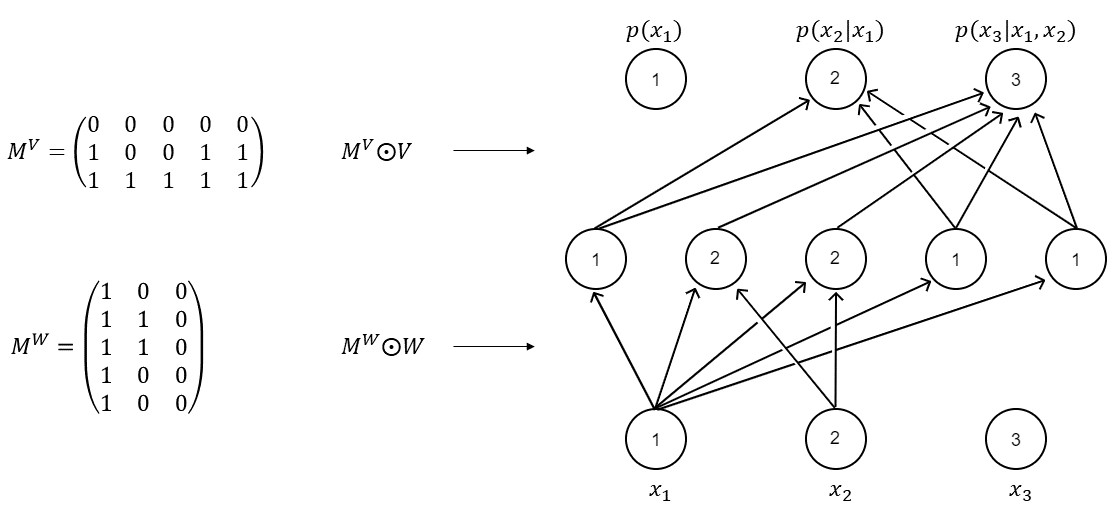
\includegraphics[width=\linewidth]{MADE_vis.jpg}
	\caption[Illustration of MADE]{Illustration of the effect of masking matrices on the graph structure of an autoencoder. The digits inside the hidden layer nodes are the $m(k)$ values that were used to calculate $\mathbf{M}^W$ and $\mathbf{M}^V$, the digits inside input / output nodes indicate the ordering. Connections where the masking matrix is 0 are dropped while others are retained (own figure).}
	\label{fig:MADE}
\end{figure}

\paragraph{Advantages of MAF}
\noindent A main disadvantage of MADE is that the order of the conditionals has a large impact on the quality of the learned density. With the correct order it may be possible to learn the density perfectly while for other orders this is not the case. To remedy this, MAF stacks $L$ MADEs and models the random numbers which are used by the MADE in layer $l$ with the model in layer $l+1$ and so on, until the random numbers of the model in the last layer are modeled by a standard Gaussian. Although each individual MADE unit has unimodal conditionals the authors of MAF argue that such a model can learn multimodal conditionals \cite{papamakarios_masked_2017}. According to them, this added flexibility improves model fit.

The central idea behind MAF is, that the distribution to be learned is viewed as a transformation of a base density $\pi_{u} (\pmb{u})$ to the target distribution via a differentiable and invertible transformation $f$. The base density should be simple in the sense that $\pi_{u} (\pmb{u})$ can be easily evaluated for all inputs $\pmb{u}$. For example the standard multivariate Gaussian where $\pmb{u} \sim \mathcal{N}(0, I)$ is a common choice. This means that $f$ takes an input $\pmb{u}$, which follows the base density distribution $\pmb{u} \sim \pi_{u} (\pmb{u})$ and transforms it to data space via the invertible function $\pmb{x}=f(\pmb{u})$. As $f$ is invertible it holds that $\pmb{u} = f^{-1}(\pmb{x})$, and the density $p(\pmb{x})$ can be calculated as

\begin{equation}
	\label{func:maf}
	p(\pmb{x}) = \pi_{u} \bigl(f^{-1}(\pmb{x})\bigr) \biggl\lvert \det \left(\frac{\partial f^{-1}}{\partial \pmb{x}} \right) \biggr\rvert.
\end{equation}

\noindent According to Papamakarios et al. \cite{papamakarios_masked_2017} the computation of this expression is tractable by design. The first part is easy to compute because $f$ is by design invertible and the base density can be evaluated for any input. The absolute determinant of the Jacobian is tractable, because the Jacobian matrix is triangular. This is due to the autoregressive property where the d-th variable $x_d$ only depends on the prior $d-1$ variables $x_{1:d-1}$. Consequently, the Jacobian of $f^{-1}$ is zero for all variables that this variable does not depend on. %TODO: Maybe add further explanation/Terms from og paper.
In each layer the mean and the log standard deviation of the d-th conditional given only the previous previous variables are computed via functions which are implemented as MADE units. Stacking multiple such units on top of each other is possible because if $f_1$ and $f_2$ are differentiable and invertible functions their composition $f_1 \circ f_2$ is also invertible and differentiable. This means the necessary properties to keep expression \ref{func:maf} tractable are maintained, even when stacking multiple layers. The use of masking makes it possible to compute the density $p(\pmb{x})$ of data $\pmb{x}$ in a single forward pass.

\paragraph{Conditional MAF}
At test time this allows to take a set of samples and produce for each of those samples the likelihood of the observed data. For reasons of numerical stability during training and testing, the log likelihood (natural logarithm) is used in this work. It is important to note here, that obtaining a single density from a sample is not yet what we want to achieve. The final goal of MAF in this use case is to obtain the observation model from it. For this, the likelihood of observed sensor data given the system state should be computed.

That is, from the set of labeled training pairs $p(\pmb{x}|y)$ should be computed instead of computing $p(\pmb{x})$. According to Papamakarios et al. \cite{papamakarios_masked_2017} this extension to handle class information $y$ comes naturally in MAF. It is obtained by conditioning each term in the chain rule decomposition of the joint probability on the available class information $y$. This means that $p(\pmb{x}|y)$ decomposes into $p(\pmb{x}|y) = \prod_{i}^{} p(x_i|x_{1:d-1},y)$. The additional class information is added to the input as a one hot encoded class vector. This information is then used by each layer as an additional input to the raw data. As the class information is given at every time step no connections need to be masked from the class inputs to the remainder of the network, since this does not violate the autoregressive property. For this work conditional MAF was employed exclusively, as all of the three datasets used for evaluation contain labeled data and conditional MAF was shown to significantly outperform unconditional MAF if labeled data is available \cite{papamakarios_masked_2017}.


\chapter{Related Work}
\label{cha:rel}

While it has been an active research topic for many years, the field of neurosymbolic AI has recently gained renewed traction after calls for more explainable and semantically sound AI systems have gotten louder \cite{garcez_neurosymbolic_2020}. This section gives a concise overview of recent developments in this field and introduces successful models related to the presented work.
Intellectually closest to this thesis is the approach proposed by Rueda et al. \cite{rueda_combining_2019}. They present the idea of using deep neural architectures as the observation model required by CSSMs. In particular the authors use a CNN to learn from time-series sensor data provided by inertial measurement units (IMUs), and predict the observed action class. In that sense the purpose of the system is very similar to the model presented here. The authors evaluated their model on the same Carrot data set that will be used for evaluation in this thesis and found that the model performance was comparable to that of state of the art deep models at the time. In the line of this work, a similar approach will be taken. With the difference being, that the observation model is obtained by a neural density estimator like MAF. The benefit of this approach over using a CNN is that MAF actually learns a distribution and can compute the density of sensor data in a single forward pass. While a CNN is a discriminative model, which computes as surrogate the predicted action from sensor data, a generative model like MAF computes the joint probability of data and labels. This fact allows the computation of the observation model $p(y_t|x_t)$ directly. Subsequently, this observation model is combined with CCBM to perform probabilistic inference. As the same dataset is used for evaluation in this thesis and the work introduced above, it will be interesting to compare the results with this approach.

Next to this, many other approaches to combine deep neural architectures with symbolic reasoning have been proposed in recent literature. DeepProbLog \cite{manhaeve_deepproblog_2018} is introduced as a framework which combines neural networks and probabilistic-logical modeling via the existing language ProbLog \cite{raedt_problog_nodate}. This is done by extending ProbLog with neural predicates. These special predicates essentially compute the probability of atomic expressions in a probabilistic logic via a neural network. The evaluation of DeepProbLog shows that this framework is capable of performing symbolic reasoning as well as deep learning from examples in an end-to-end fashion. The benefit of this system over previous work is, that it integrates neural networks into a probabilistic-logical framework instead of approximating reasoning with neural nets. Consequently, the resulting model is able to perform probabilistic-logical inference, deep learning and combinations thereof. The downside of this approach is that its inference algorithms and language are ill-suited for dynamic systems, such as HAR.

Another hybrid architecture for HAR in an order-picking scenario is proposed by L\"udtke et al. \cite{ludtke_human_2021}. This model first predicts higher level movement descriptors from sensor data via a temporal convolutional neural network. These attributes are then used by a shallow classifier to estimate the most likely activity class. Additionally, the current process step can be taken into account as context information by making it accessible to the shallow classifier. One main benefit of this system is that it allows the integration of prior context information without re-training the entire network. Consequently, the deep model can be interpreted as a tool for feature extraction from sensor data. This means that it is largely domain independent and only the shallow prediction head has to be adjusted when switching domains. This model is reported to achieve state-of-the-art HAR performance even in the absence of context information, but performance increases further if relevant information from the process step is included, even if it is not always correct.

A very recent approach that shows promising results for HAR is DUSTIN \cite{arrotta_knowledge_2022}, which employs knowledge infusion on top of features extracted via a neural network. That is, the model uses a CNN to extract features from time series sensor data as well as the high-level context and concatenates to this representation a set of features which are obtained by a knowledge based reasoner before its classification layer. Just as for CSSMs, this has the added benefit that common-sense knowledge can be introduced to the model, which means that estimated action sequences are consistent with the user-context. However, unlike most models DUSTIN allows infusion of additional knowledge into the deep model itself. That is instead of applying such information before or after the learning process, additional knowledge from a symbolic reasoner is added before the classification layer of the deep model. This is achieved by aggregating raw context data (e.g. the GPS data of the user) to high level context data (e.g. the users semantic location in the world). From this, the symbolic reasoner produces only activities which are consistent with the observed context (e.g. if the user is at a library, they are not doing sports). The evaluation of DUSTIN shows that it is able to outperform other state-of-the-art neuro-symbolic approaches while achieving a high sample efficiency. In comparison with other hybrid approaches that employ knowledge infusion \cite{bettini_caviar_2020, sukor_hybrid_2019}, DUSTIN is the first HAR model to apply the knowledge infusion \emph{within} the deep model instead of applying it before or after the learning process.


\chapter{Methods}
\label{cha:alg}

At its core, the hybrid model proposed in this paper consists of three main components which can be exchanged with other methods and combined in a modular way. Figure \ref{fig:schema} illustrates a schematic of these components and their interactions. Ultimately, the goal of the hybrid model is to achieve sate-of-the-art HAR performance with increased sample efficiency compared to approaches which solely rely on deep learning methods. To this end three components are defined which can be altered to investigate the effects of each component.

\begin{figure}[h]
	\centering
	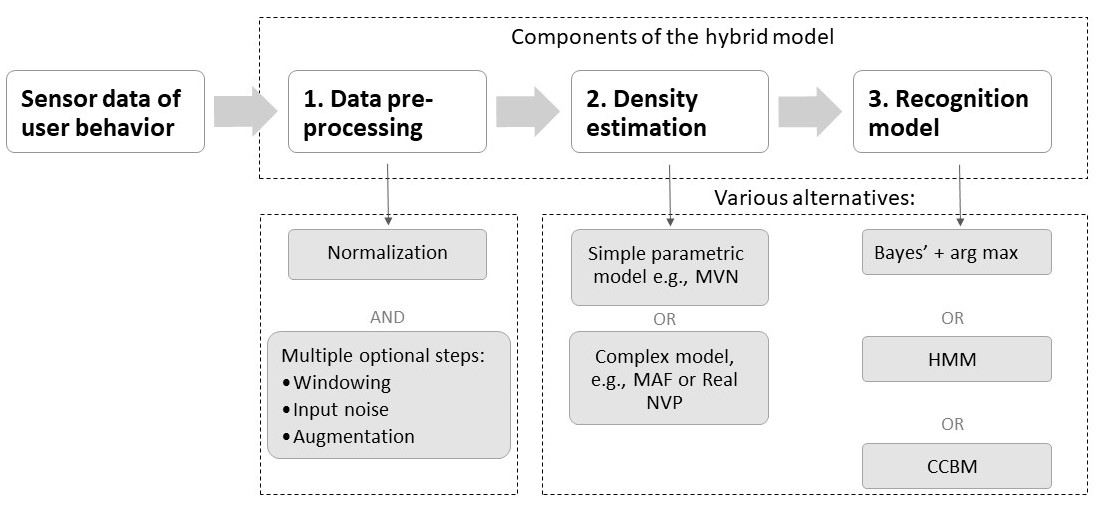
\includegraphics[width=\linewidth]{Hybrid_V2.jpg}
	\caption[Hybrid architecture components]{Components of the hybrid architecture and some of their possible variations (own image).}
	\label{fig:schema}
\end{figure}

\noindent First is the data pre-processing stage in which numerical raw data is read and processed. Various steps can be undertaken here to make the training of the following module more robust. Secondly, a method for density estimation is employed to obtain sample densities. The third and last step in this process is the recognition model which may use the obtained densities directly for activity recognition or as an observation model for more complex models. From this the concrete prediction of an activity class or state is obtained. The remainder of this chapter introduces each component and the implementation thereof in greater detail. Furthermore, some other models choices for these components are discussed briefly.

\section{Data Pre-Processing}
\label{sec:prep}

The data of all three datasets used in this work stems from inertial measurement units (IMUs) which measure acceleration and angular rates. MotionSense \cite{malekzadeh_mobile_2019} and the UCI HAR \cite{anguita_public_2013} dataset use the accelerometer and gyroscope sensors of smartphones, while the Carrot dataset \cite{kruger_recognising_2011} uses standalone IMUs which are located in 5 different locations on the body. Furthermore, the UCI HAR dataset has pre-computed features while the remaining two contain raw sensor data. As UCI HAR is already pre-processed it was chosen not to employ any methods that alter this default pre-processing of the UCI HAR dataset. Thus, the processing steps below are applicable to the Carrot and MotionSense datasets only. In terms of pre-processing several steps were undertaken and their effects are evaluated in section \ref{sec:results} of this thesis. Normalization is always done for both datasets, as without it the training of the MAF is unstable. In addition to this mandatory step, three optional pre-processing steps may be employed for both datasets. These steps are windowing, augmentation, and noise addition. It is possible to select a subset of these operations, including none or all of them together.

\paragraph{Normalization}
To begin with, each channel in the data is normalized to the interval $[0,1]$. This is achieved by fitting a \emph{MinMaxScaler} to the training data, the same transformation with this scaler is then applied to the test and validation data to normalize it in the same way. Also tested was z-score normalization per channel, but it quickly became apparent that training was more stable with the \emph{MinMaxScaler}.

\paragraph{Windowing}
The process of windowing, segments the raw data into windows of a specified window size \emph{T}, using a step size of \emph{s}, indicating by how many samples to step the subsequent window. Note, that window size and step size can be used to create overlapping windows. If $s=T$ no overlap occurs, if for example $s = \frac{T}{2}$, subsequent windows have an overlap of 50 \%. Such overlap creates more samples than windowing without it. The class of a window is the majority class of its components. It is apparent that with a window size of $T=1$ the notion of a sample (i.e., a data point at a single time step) and a window agree. For simplicity, a data window of arbitrary size will be referred to as a \emph{sample} in the remainder of this thesis.

The idea behind windowing the data is that actions in reality have a duration that is typically much greater than the sampling rate of the sensors. Thus, many individual time steps can be segmented together in order to obtain a sample which corresponds to a real-world activity. Thus, such a segmentation is typically done for HAR applications. The UCI HAR dataset is segmented by default into windows of size $T=128$.

\paragraph{Data Augmentation}
Next to windowing, two simple data augmentation methods can be used to augment the training data. These are adapted from the paper on data augmentation methods for sensor data by Um et al. \cite{um_data_2017}. Namely jittering and scaling of data are employed subsequently. If used, a proportion of the training data, i.e., from 0 to 100 \% is added to the original data in a slightly altered fashion to increase the number of training samples. The employed augmentation methods are jittering, that is adding Gaussian noise with $\mu = 0, \sigma = 0.05$, and scaling, that is scaling each channel by multiplying with a factor drawn from a normal distribution with $\mu = 1, \sigma = 0.1$. This step was added as an option because the amount of training data is often very limited.

\paragraph{Input Noise Injection}
To combat overfitting of the subsequent MAF module another option was introduced: Adding noise directly to the raw data. If this option is set, Gaussian noise with $\mu = 0, \sigma = 0.025$ is added to training samples. The idea here is, that this does not change the samples enough to where they would be considered a different class, but enough that some of the interpersonal variability between how different subjects perform certain activities is captured. Adding noise differs from the data augmentation option where the original data is left unchanged and only augmented samples are added to the training data. It is also possible to use both mechanisms at the same time.

\paragraph{Pre-Processing Alternatives}
One of the main difficulties of HAR lies in the fact that different subjects often produce greatly differing sensor readings for the same activity. That is a high intra-class variability is present in HAR datasets. This is a consequence of various physiological differences between subjects. Factors such as variances in age, height or weight can impact how actions are performed, and thus sensor readings, strongly. Consequently, it is preferable for HAR tasks to have a dataset that captures most of this variability in its training set by containing data of many different subjects. However, labeled motion data is often hard to obtain. To counteract this, the pre-processing component of the hybrid model could be refined further. For example, more advanced augmentation methods, such as the ones proposed by Um et al. \cite{um_data_2017}, are available. These aim to combat a lack of labeled data. Furthermore, representation learning from unlabeled time series data in a self-supervised manner as proposed by Eldele et al. \cite{eldele_time-series_2021} may be an interesting research direction. In this way helpful representations can be learned which are useful for the downstream task of recognizing human activities.

\section{Density Estimation}
\label{sec:densest}

The second component of the proposed hybrid system is the density estimation component. This module computes the probability density of samples which can be used later on in the recognition model either to build the observation model or to predict actions from conditional densities directly. Just like the other two modules, many concrete implementations exist for this component.

\paragraph{Multivariate Normal Distribution}
Potentially the simplest method of density estimation is a parametric model for which the probability densities can be computed easily. An example of this is the multivariate normal (MVN) distribution. For this thesis one MVN per activity class $y$ was fitted for benchmarking purposes. Thus a set of MVNs with unconstrained covariance matrices allow conditional density estimation. Each MVN can be used to obtain the density $p(\pmb{x}|y)$ of a sample, conditioned on activity class $y$.

\paragraph{Advanced Density Estimation Methods}
However, there are more sophisticated methods of obtaining probability densities from samples. One such method is density estimation based on neural networks such as the previously discussed MADE and MAF models. The goal of the neural architecture of the hybrid system is to obtain a likelihood from given sensor data which is useful for the downstream task of recognizing human activities. As MAF has shown promising performance in density estimation tasks \cite{kobyzev_normalizing_2021} it was elected for the implementation of this component. At its heart, MAF is trained on data to fit the assumed true data distribution from samples. As discussed in section \ref{sec:maf}, MAF calculates densities of samples within a single forward pass, which makes obtaining densities with a trained MAF computationally inexpensive. It was chosen to use a conditional MAF as the density estimation component of the hybrid model. To build this model a base implementation of MAF in PyTorch \cite{kostrikov_pytorch-flows_2022} was used and heavily adapted to fit the requirements of this thesis. Each Layer of the MAF consists of a MADE followed by a Batch normalization layer. The MADE uses the ReLu activation function. The number of MAF modules that are stacked on top of each other is a tunable hyperparameter. However, five blocks of the above architecture provided the most promising results in many of the experiments.

MAF is trained by minimizing the negative log likelihood (NLL) loss, over a number of max epochs which can be set as a hyperparameter. The best model is selected by the lowest loss on the validation data. Since, the downstream task is the goal of recognizing activities it was also tested to select the best model according to recognition accuracy. However, in most cases these two methods of selecting the best model agree or differ only marginally. Therefore, minimizing the NLL loss was chosen as a suitable mechanism for model selection. Furthermore, it is important that training samples are shuffled to ensure that they are independent and identically distributed. If this is not done, most batches only contain samples from one class and MAF tends to learn unimodal or other very simple distributions.

In theory other generative models can be employed in a very similar fashion to obtain (conditional) densities of samples. Another notable neural method that can be used for density estimation and is also based on invertible flows is Real NVP \cite{dinh_density_2017} or extensions thereof like Glow \cite{kingma_glow_2018}.

\section{Recognition Model}
The last component of the proposed hybrid model is the recognition model. The goal of this model is to accurately recognize human activities given the output of the previous step. To achieve this, many concrete options are applicable. The following paragraph will introduce three of the potential mechanisms.

\paragraph{Bayes Classifier}
The simplest recognition model is to compute $p(y_c|\pmb{x})$ for each class $c \in C$ via Bayes' theorem and then predicting the most probable class via the $\argmax$ operation. This mechanism is known as a Bayes classifier and is implemented for this work as follows: At test time the set of test samples is passed through the MAF and the $\log p(\pmb{x}|y)$ of each sample is computed. To obtain a prediction of activities from these densities the log density of sample $\pmb{x}$ conditioned on each individual class $c \in C$ is calculated using the MAF. As discussed in section \ref{sec:maf}, the $\log p(\pmb{x}|y_c)$ for class c is obtained with a single forward pass of the sample through the MAF, which makes estimation of sample densities fairly cheap. By doing this for all classes, a matrix containing the logarithmic density of each test sample for each of the classes is computed. From there Bayes' theorem is used to calculate $p(y_c|\pmb{x}) = \frac{p(\pmb{x}|y_c) \cdot p(y_c)}{p(\pmb{x})}$. As $p(\pmb{x})$ is the same within each sample $\pmb{x}$, the denominator is a constant factor per test sample. Hence, it can be left out to achieve a proportional result which suffices for predicting the most probable class. The prior $p(y_c)$ for all classes $c$ is easily computed as the class distribution of training samples. As operations occur in log space, the numerator of Bayes' theorem is obtained by adding the values $\log p(\pmb{x}|y_c) + \log p(y_c)$. For the prediction itself, the most probable class can be predicted by getting the $\argmax$ over all classes y for each sample.

\paragraph{Hidden Markov Model}
The previously described method however does not take into account the any other prior information that might be available such as the temporal structure of actions. To include such knowledge other methods of estimating states from observations are better suited. For example the simple Bayesian recognition model could be exchanged for a hidden Markov model (HMM). A HMM is fully specified by its transition model, emission probabilities and a prior distribution of states. In this recognition model the emission probabilities of an HMM are obtained by the distribution over activity classes given the observation at time $t$. This is obtained as a result of the density estimation component. The transition model can be computed empirically from the observation data by counting how often each state follows each other state, resulting in an $M \times M$ matrix where $M$ is the number of distinct states of the HMM. Likewise, the prior is obtained by measuring state frequencies from data. To perform the filtering task at time t, i.e., estimating the probability of a state given all observations up to this time, the prediction (equation \ref{func:p}) and correction (equation \ref{func:c}) steps introduced in section \ref{sec:cssm} are employed. By doing this sequentially, a trajectory of the most probable states can be obtained which is the recognition of the individual activities as required by HAR.

\begin{align}
	p(x_t|y_{1:t-1}) &= \sum_{x_{t-1}} p(x_t|x_{t-1}) p(x_{t-1}|y_{1:t-1}) \label{func:p} \\
	p(x_t|y_{1:t}) &= \frac{p(y_t|x_t) p(x_t|y_{1:t-1})}{p(y_t|y_{1:t-1})} \label{func:c}
\end{align}

\paragraph{Computational Causal Behavior Models}
Conceptually, activity recognition using CCBM works the same way as for an HMM. The difference lies in how the transition model of states is obtained. In CCBM the transition probabilities between actions are computed following the model presented in equation \ref{func:ccbm} of this work. The use of CCBM as the recognition model is especially sensible if the sequence of actions to be recognized follows some goal directed behavior. This is for example the case in the Carrot data set. In contrast to the exact inference in the paragraph explained above, CCBM typically uses approximate filtering algorithms as state spaces get large quickly. In such spaces the marginal filter has been shown by Nyolt et al. \cite{nyolt_marginal_2015} to be an effective method of performing the filtering task. To perform activity recognition using CCBM, first the observation model is obtained from the density estimation component. Following this, the observation model is then compiled with the action templates, initial and goal states into a marginal filter. Using this filter, a trajectory of the most probable activity states can be computed.

\chapter{Experimental Evaluation}
\label{cha:exp}

\section{Datasets}
\label{sec:data}
The three datasets used in the evaluation of this work are the Carrot \cite{kruger_recognising_2011}, MotionSense \cite{malekzadeh_mobile_2019} and UCI HAR \cite{anguita_public_2013} datasets. All three sets contain measurements from inertial measurement units. The individual datasets are introduced in greater detail in the paragraphs below. An overview of the dataset statistics can be found in table \ref{tab:sets}.

\begin{table}[H]
	\footnotesize
	\centering
	\begin{tabular}{l c c r r r r}
		\toprule
		\textbf{Dataset} & \textbf{Classes} & \textbf{Channels} & \textbf{Train} & \textbf{Valid} & \textbf{Test} & \textbf{Subjects} \\
		\midrule
		Carrot & 16 & 30 & 146570 & 36643 & 30036 & 7 \\
		MotionSense & 6 & 12 & 812035 & 315156 & 285674 & 24 \\
		UCI HAR & 6 & 561 \tablefootnote{561 is the number of pre-computed features used for training. The number of actual sensor channels is 6.} & 5881 & 1471 & 2947 & 30 \\
		\bottomrule
	\end{tabular}
	\caption[Dataset statistics]{\label{tab:sets} Dataset statistics}
\end{table}

\paragraph{Carrot}
The Carrot dataset uses standalone IMUs which are attached to the subject its body in five locations: upper torso, left forearm, right forearm, left calf, right calf. Seven subjects were tasked with a typical activity of daily living to produce this data.
The task was to prepare, cook, serve and eat a carrot soup. Afterwards, cleaning up and washing the dishes was required. During this task, acceleration and angular rates were measured with the IMUs and annotated based on a motion capturing system.
It contains 16 action classes and additionally more fine grained annotations of objects and places. However, this work only uses the 16 action classes as labels. The data is recorded at a sampling rate of 120 Hz. Each sensor at each of the five locations records the angular rate and acceleration in x,y and z direction. Thus, the dataset consists of $D = 5 \cdot 6 = 30$ channels.

\paragraph{MotionSense}
The MotionSense dataset includes time-series data generated by accelerometer and gyroscope sensors. Attitude, gravity, acceleration, and rotation rate are measured on the x,y and z axis. Consequently, this dataset has $D = 4 \cdot 3 = 12$ channels. The data was collected with the sensors of an iPhone 6s. Only a single location of the sensor was taken into account, which is the front pocket of the subject. Data was collected at a sampling rate of 50 Hz. In total, the data stems from 24 subjects with differing physiological properties. They performed six activities in 15 trials: downstairs, upstairs, walking, jogging, sitting, and standing.

\paragraph{UCI HAR}
The UCI HAR dataset is slightly different as it is already processed and contains pre-computed features. Acceleration and angular rates were measured along the x,y and z axis at a sampling rate of 50 Hz, resulting in $D = 2 \cdot 3 = 6$ channels. All data was recorded with smartphone sensors from a Samsung Galaxy S II positioned at the waist. Data was labeled manually via video recordings. The pre-processing of this dataset segments data into windows of 2.56 s (i.e., 128 samples) with 50 \% overlap. The acceleration signal was then separated into a body acceleration and gravitational component using a Butterworth low-pass filter. Afterwards 561 distinct features from the time and frequency domain of the raw signals were calculated from each segment. In total, 30 subjects ranging in age from 19 - 48 years performed six activities: walking, upstairs, downstairs, sitting, standing and laying.


\section{Experiments}
\label{sec:exp}
To evaluate the usefulness of neural density estimation methods for HAR applications several experiments were conducted on the previously introduced datasets. From the set of optional pre-processing steps, five tunable parameters are obtained. Three boolean flags can be set for windowing ($W$), augmentation ($A$), and input noise injection ($N$). If windowing is true, some window size $T \geq 2$ needs to be specified. In this case, also a step size $s$ with $1 \leq s \leq T$ should be given for stepping the segments in the training data. In the experiments presented here, the step size is fixed to $s = \frac{T}{2}$ such that the training data segments have an overlap of 50 \%. Validation and testing sets use segmentation without overlap by default. If windowing is false, this indicates that no explicit windowing is performed, or in other words window size $T = 1$. The two remaining boolean flags $A$ and $N$ control whether the augmentation of training data, respectively the input noise injection as described in section \ref{sec:prep} is performed. Various combinations of these parameters for each dataset have been selected and evaluated. The hyperparameters of these methods which control the amount of noise added and scaling done are the default settings used in the implementation of data augmentation for wearable sensor data \cite{um_augmentation_2017}. In particular, the usefulness of MAF as the density estimation component is evaluated and compared to the baseline method of estimating densities with a MVN per activity class as described in section \ref{sec:densest}. For this evaluation, the average log likelihood obtained over all test samples is reported. As the downstream task is the recognition of activities, two different components for the density estimation component are compared using two different recognition models. More precisely, the recognition accuracy of both MVN and MAF densities are compared using the Bayes classifier and an HMM as the two recognition models. The results of all experiments are reported in section \ref{sec:results}.

\paragraph{Train-Test Split}
To facilitate an evaluation that is as close to a real world scenario as possible, a leave-one-subject-out strategy was employed for splitting the data into test and training set. Realistically, the model would be trained on some data and each new subject would not have its data in the training set. This fact is emulated by leaving one or more subjects completely out of the training set and using this subject for testing. This strategy was employed for the Carrot and MotionSense datasets, for the UCI HAR dataset the predefined train-test split was used which also leaves a set of subjects completely out of the training set. For the Carrot dataset it was decided arbitrarily that subject 7 would be the test subject and the remaining data would be used with a 70 \% - 30 \% split for training and validation. The MotionSense data was split in such a way that subjects 1 to 14 are used for training, 15 to 19 for validation and  20 to 24 as test subjects. UCI HAR splits the data such that 56 \% of subjects are used for training, 14 \% for validation and 30 \% for testing.

\paragraph{Settings}
All experiments are conducted with a five layer MAF, the number of hidden neurons in each MADE Layer is $H=512$. Model parameters are updated by minimizing the negative log likelihood over the training data. The Adam optimizer is used with a base learning rate of $\lambda = 5 \times 10^{-5}$ and a weight decay of $d = 1 \times 10^{-6}$. Furthermore, the batch size is set to $bs = 128$. The model was trained on a commercial computer utilizing the PyTorch framework with CUDA enabled on a single NVIDIA RTX 2070 SUPER GPU.


\section{Results}
\label{sec:results}

\subsection{Carrot Dataset}
Table \ref{tab:2eps} shows the results of experiments on the Carrot dataset, where MAF was only trained for 2 epochs. The individual settings regarding the optional pre-processing steps can be read off the table.

\begin{table}[H]
	\centering
	\tiny
	\begin{tabular}{c l c c c c c c c c c c}
		\toprule
		\multirow{2}{*}{\bfseries Dataset} & 
		\multirow{2}{*}{\bfseries W} & 
		\multirow{2}{*}{\bfseries T} &
		\multirow{2}{*}{\bfseries s} &
		\multirow{2}{*}{\bfseries A} &
		\multirow{2}{*}{\bfseries N} &
		\multicolumn{2}{c}{\bfseries LL} & 
		\multicolumn{4}{c}{\bfseries Accuracy}\\
		\cmidrule(lr){7-8}
		\cmidrule(lr){9-12}
		& & & & & & MVN & MAF & MVN + Bay. & MAF + Bay. & MVN + HMM & MAF + HMM \\
		\cmidrule(lr){1-12}
		%------
		CARROT &   F &       1 &       1 &    F &  F &   65.5 &   \textbf{68.2} &   \textbf{0.6006} &   0.5384 &   0.6005 &   0.5381 \\
		CARROT &   F &       1 &       1 &    F &  T &   59.4 &   \textbf{59.7} &   0.5932 &   \textbf{0.6037} &   0.5927 &   0.6034 \\
		CARROT &   F &       1 &       1 &    T &  F &   54.8 &   \textbf{68.2} &   \textbf{0.5683} &   0.5624 &   0.5680 &   0.5621 \\
		CARROT &   F &       1 &       1 &    T &  T &   48.3 &   \textbf{59.2} &   0.5103 &   0.6166 &   0.5101 &   \textbf{0.6202} \\
		CARROT &   T &      26 &      13 &    F &  F & \textbf{2988.3} & 1555.2 &   \textbf{0.3299} &   0.3290 &   0.3299 &   0.3290 \\
		CARROT &   T &      26 &      13 &    F &  T & \textbf{2018.9} & 1416.1 &   \textbf{0.4398} &   0.3861 &   0.4398 &   0.3887 \\
		CARROT &   T &      26 &      13 &    T &  F & \textbf{1883.5} & 1720.2 &   \textbf{0.4312} &   0.4121 &   0.4312 &   0.4130 \\
		CARROT &   T &      26 &      13 &    T &  T & \textbf{1569.2} & 1513.4 &   0.4909 &   \textbf{0.5351} &   0.4900 &   0.5342 \\
		CARROT &   T &       8 &       4 &    T &  F &  534.0 &  \textbf{695.9} &   0.3759 &   0.5341 &   0.3713 &   \textbf{0.5344} \\
		CARROT &   T &      64 &      32 &    T &  F & 1378.6 & \textbf{3319.6} &   0.1215 &   \textbf{0.4030} &   0.1215 &   0.4030 \\
		\bottomrule
	\end{tabular}
	\caption[Evaluation results Carrot, short]{\label{tab:2eps} Log likelihoods and recognition accuracies of MAF and a baseline MVN trained per class with unconstrained covariance matrix. The settings of the experiments are reported in the first six columns, the results in the remaining six. MAF was trained for a maximum of 2 epochs.}
\end{table}

\paragraph{Comparing MVN and MAF}
\noindent The first result that becomes apparent is that MAF achieves higher likelihoods if the data is not windowed or window sizes are relatively small. This result is expected, as MAF is a much more flexible model than a set of MVN conditioned on the class. MAF should in theory be able to fit an arbitrary distribution while MVN is expected to only be a good fit if individual features are (approximately) normally distributed. Given this discrepancy in log likelihood (LL) it is surprising that MVN significantly outperforms MAF in the base case where no windowing, augmentation or noise injection is done. In that case MVN achieves a LL of 65.5 while that of the MAF is 68.2. Nevertheless, MVN achieves the higher recognition accuracy at 60.06 \%, an increase of 6.22 percentage points (pp) from the result of MAF at 53.84 \%. This outcome warrants the investigation into the Carrot dataset to check if features may indeed be normally distributed which could explain the good performance of the MVN.

To examine this, a $30 \times 30$ pair plot was drawn, which plots a histogram per feature from $1600$ samples of the Carrot data and compares each feature to all others. This plot can be found in appendix \ref{cha:appendix-b}, the script to generate it is contained in the attached code. The plot shows that circa half of the 30 features from the Carrot dataset are somewhat well represented by a normal distribution. Given this result, the fact that a MVN performs well is less surprising. Still, the overall recognition accuracy is relatively low at around 60 \%. This can be explained by the fact that the Carrot dataset is difficult to learn from.

\paragraph{Challenges of the Carrot Dataset}
The first challenge of the Carrot dataset is, that it is relatively small. Data stems from only 7 subjects and the number of total (non-windowed) training samples is also low at 146570. As discussed in section \ref{sec:prep} a low number of training subjects might lead to difficulties during the learning process due to the high intra-class variability in HAR tasks. In that sense it is plausible that a less flexible model can achieve better results simply because it cannot overfit to the training data as much. Thus, it may generalize better to sensor readings from unseen subjects which perform activities slightly differently from the training data subjects. The second difficulty of the Carrot data is that some activities occur much less frequently at a shorter duration or have many different concrete expressions. To support this argument let us look at two activities that are hard to recognize in greater detail.

Figure \ref{fig:conf} shows the confusion matrix of the Bayes classifier using MAF densities and illustrates these examples. The activity \emph{stand up} for example has the lowest relative frequency in the dataset at 0.36 \%. Also the duration of that activity is typically very short. At prediction time it is often confused with other activities that are more frequent. The activity \emph{put} is the third most frequent (11.51 \%) in the training data, but still recognizing it accurately seems difficult. The confusion matrix shows that it has a large spread of other activities that is is confused with at test time. A plausible explanation for this observation is that \emph{put} can have various expressions, which differ greatly in the sensor readings they produce: Putting a glass in a cupboard above your head produces different measurements from putting a dish in the sink at waist level. Other activities follow a more strict pattern. It is also interesting to see that \emph{put} is often confused with the activity \emph{eat}. Interpreting eating as putting food in ones mouth may help to explain this pattern. Similarly, \emph{put} and \emph{take} are often confused for each other which is also an intuitive result as they share much of the same motion patterns. The result that the Carrot dataset is difficult to train on is supported by other researchers as well. For example Rueda et al. \cite{rueda_combining_2019} report an overall activity recognition accuracy on subject 7 of the Carrots data of 65.2 \% using a CNN. However, the recognition accuracy of the activity \emph{put} is only 35.1 \% and that of \emph{stand up} is 11.7 \%.

\begin{figure}[h]
	\centering
	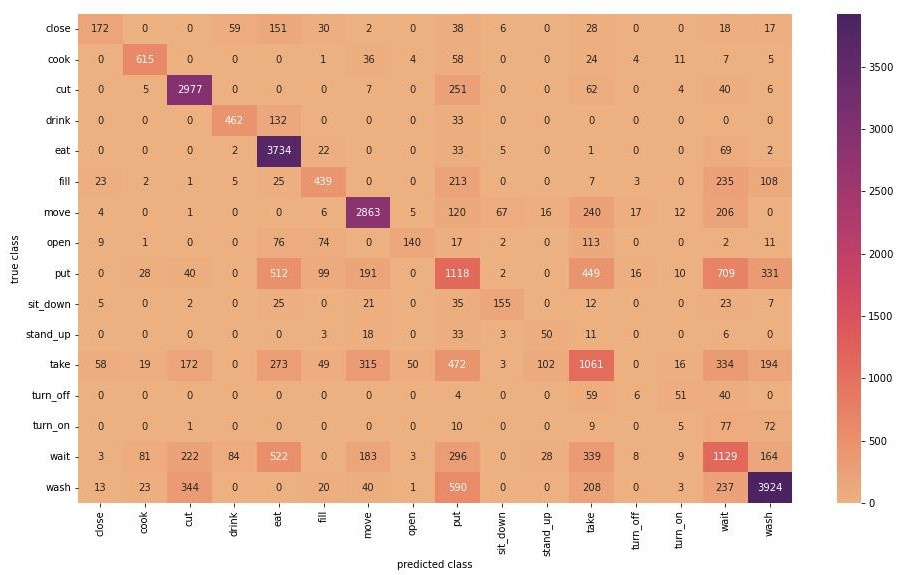
\includegraphics[width=\linewidth]{conf_mat.jpg}
	\caption[Confusion matrix Carrot]{Confusion matrix of the Bayes classifier on MAF densities with settings W=False, A=True, N=True (own image).}
	\label{fig:conf}
\end{figure}

Due to the lack of subject variety and class imbalance, generalization performance on data from unseen subjects is poor. MAF has the tendency to overfit easily to a few or only one of the most frequent classes on the Carrot dataset. This behavior was observed early during the development of the model presented here. In fact, when optimizing the model parameters with a large initial learning rate or using a more complex MAF with a greater number of hidden neurons or layers, a severe case of mode collapse is observed. That is, the model learns an unimodal density which only assigns plausible densities to one class and the conditional densities for all other classes are infinitesimally small. To counteract this, a small initial learning rate and a sufficient but not too large number of hidden neurons needs to be chosen for training MAF.

\paragraph{Effectiveness of Pre-Processing}
Even with a suitable hyperparameter configuration, MAF tends to overfit on the Carrot data. Table \ref{tab:100eps} shows the results of the experiments where MAF was trained for a maximum of 100 epochs and supports this claim. It can be observed that without any additional measures to combat overfitting, the accuracy diminishes significantly compared to the results presented in table \ref{tab:2eps} where the MAF was only trained for two epochs. Thus, the effect of input noise injection and data augmentation is evaluated. Especially the addition of noise appears to counteract the overfitting effectively. Being such a simple measure it is able to not only stop the decrease in accuracy but allows for a more robust learning process where the performance actually increases over time. On its own, data augmentation does not increase recognition performance but in combination with noise the best results on the Carrot data are achieved at a recognition performance of 62,76 \%.

\begin{table}[ht]
	\centering
	\tiny
	\begin{tabular}{c l c c c c c c c c c c}
		\toprule
		\multirow{2}{*}{\bfseries Dataset} & 
		\multirow{2}{*}{\bfseries W} & 
		\multirow{2}{*}{\bfseries T} &
		\multirow{2}{*}{\bfseries s} &
		\multirow{2}{*}{\bfseries A} &
		\multirow{2}{*}{\bfseries N} &
		\multicolumn{2}{c}{\bfseries LL} & 
		\multicolumn{4}{c}{\bfseries Accuracy}\\
		\cmidrule(lr){7-8}
		\cmidrule(lr){9-12}
		& & & & & & MVN & MAF & MVN + Bay. & MAF + Bay. & MVN + HMM & MAF + HMM \\
		\cmidrule(lr){1-12}
		%------
		CARROT &   F &       1 &       1 &    F &  F &   \textbf{65.5} &   47.2 &   \textbf{0.6006} &   0.3938 &   0.6005 &   0.3936 \\
		CARROT &   F &       1 &       1 &    F &  T &   59.4 &  \textbf{ 61.4} &   0.5932 &   \textbf{0.6083} &   0.5927 &   0.6080 \\
		CARROT &   F &       1 &       1 &    T &  F &   \textbf{54.8} &   53.1 &  \textbf{0.5683} &   0.3289 &   0.5680 &   0.3293 \\
		CARROT &   F &       1 &       1 &    T &  T &   48.3 &   \textbf{60.8} &   0.5103 &  \textbf{0.6276} &   0.5101 &   0.6276 \\
		CARROT &   T &      26 &      13 &    F &  F & \textbf{2988.3} & 2860.8 &   0.3299 &   \textbf{0.4026} &   0.3299 &   0.4026 \\
		CARROT &   T &      26 &      13 &    F &  T & \textbf{2018.9} & 1951.1 &   \textbf{0.4398} &   0.3377 &   0.4398 &   0.3385 \\
		CARROT &   T &      26 &      13 &    T &  F & 1883.5 & \textbf{2965.4} &   0.4312 &   \textbf{0.4779} &   0.4312 &   0.4771 \\
		CARROT &   T &      26 &      13 &    T &  T & 1569.2 & \textbf{1972.0} &   \textbf{0.4909} &   0.3203 &   0.4900 &   0.3203 \\
		CARROT &   T &       8 &       4 &    T &  F &  534.0 & \textbf{1032.3} &   0.3759 &   \textbf{0.5125} &   0.3713 &   0.5117 \\
		CARROT &   T &      64 &      32 &    T &  F & 1378.6 & \textbf{5491.9} &   0.1215 &   \textbf{0.4051} &   0.1215 &   0.4051 \\
		\bottomrule
	\end{tabular}
\caption[Evaluation results Carrot, long]{\label{tab:100eps} Log likelihoods and recognition accuracies of MAF and a baseline MVN trained per class with unconstrained covariance matrix. The settings of the experiments are reported in the first six columns, the results in the remaining six. MAF was trained for a maximum of 100 epochs.}
\end{table}

\noindent When looking at the case where data is segmented into windows of size $T=26$ it is apparent that for short training periods augmentation, noise injection and especially the combination of both, improve recognition performance significantly from the base case. However, overall performance versus the non-windowed data is lower. This is true for predictions using MAF densities but also those using the MVN densities. A possible explanation for this is, that the increased dimensionality of windowed data makes accurate density estimation much more difficult. Models which cope well with high dimensional data and are designed as discriminative models to predict classes such as CNNs may therefore be better suited for windowed high dimensional data. To support this argument, Rueda et al. \cite{rueda_combining_2019} achieve the 65.2 \% accuracy on the Carrot dataset with a CNN on data that has been segmented into windows of size $T=128$. Setting the window size to even half that at $T=64$, does not produce promising results for MAF or MVN. Instead, increasing window size leads to a further decrease in recognition accuracy. In the case where the MAF was trained for 100 epochs only augmentation has a net positive effect on recognition accuracy over the base case. These results indicate that a small window size and thus a reduced number of dimensions may be better for estimating useful densities with MAF. Consequently, the argument can be made that for MAF to be an effective method of obtaining densities from time series data, some form of dimensionality reduction or representation learning should be applied before the training phase.

\paragraph{Comparing Bayes Classifier and HMM}
From the results it can be observed that in most cases the recognition accuracy when using the simple Bayes classifier differs not or only marginally from that of an HMM. In most cases the HMM recognizes activities slightly less accurately. Two notable exceptions to this can be found in table \ref{tab:2eps}, where the HMM outperforms the Bayes classifier slightly, using MAF densities. Generally, the likelihoods provided by MVN and MAF on the Carrot dataset are high for the most common activity, regardless of the true class of a sample. This is illustrated in table \ref{tab:llc}. It shows the average per class log likelihood of test samples grouped by their true class. That is, the first data column of that table shows the average LL per class over all test samples belonging to class zero. Consequently, we would expect that the entries on the main diagonal would be the maximum in every column. However, this is not the case. Rather a few classes, such as the majority class 15, have high likelihoods across most samples, regardless of their true class. It can be stated that on the Carrot data often highly confident but wrong predictions occur. As an example take class 12. On average, samples belonging to this class have the highest test likelihood not for that class (avg. LL is 28.2) but rather for class 14 (avg. LL is 66.5). This is a large discrepancy. Consequently, neither the prior of the Bayes classifier nor the more complex HMM recognition model have a large impact on recognition accuracy. The predicted class of a sample is mainly controlled by the calculated likelihoods. 

\begin{table}[H]
	\tiny
	\centerline{%
	\begin{tabular}{c c c c c c c c c c c c c c c c c}
		\toprule
		\multirow[b]{2}{*}{} &
		\multicolumn{16}{c}{\bfseries Avg. per class LL of samples grouped by true class y}\\
		\cmidrule(lr){2-17}
		\bfseries Class & 0 & 1 & 2 & 3 & 4 & 5 & 6 & 7 & 8 & 9 & 10 & 11 & 12 & 13 & 14 & 15\\
		\cmidrule(lr){1-17}
		0 & 40.0 & 30.3 & -28.9 & -206.4 & -97.8 & 12.8 & 20.4 & 41.3 & 7.6 & 12.7 & 1.3 & 7.3 & 23.2 & 14.6 & -2.6 & 7.5 \\
		1 & -18.1 & \textbf{70.3} & 37.1 & -36.0 & -32.5 & 5.6 & 22.6 & 10.1 & 20.4 & 10.8 & 2.8 & 15.2 & 38.7 & 16.2 & 29.3 & 9.6 \\
		2 & 10.5 & 52.2 & \textbf{70.3} & 13.7 & 12.8 & 13.5 & 13.4 & 22.1 & 24.8 & -25.0 & -5.9 & 18.4 & 25.0 & 28.7 & 33.8 & 20.0 \\
		3 & 2.2 & -32.1 & -72.2 & -34.4 & -27.5 & -8.9 & -47.8 & 1.8 & -56.7 & -41.2 & -94.2 & -43.4 & -146.7 & -64.0 & -41.9 & -65.7 \\
		4 & 19.7 & -37.1 & -19.4 & \textbf{20.5} & \textbf{38.9} & 10.4 & -37.3 & 16.4 & -17.0 & -32.4 & -22.0 & -41.4 & -120.0 & -85.6 & -24.8 & -31.2 \\
		5 & 25.3 & 50.2 & 39.9 & -223.5 & -240.7 & 32.6 & 21.6 & 35.0 & 16.0 & 14.6 & 30.2 & 10.7 & 45.7 & 44.8 & 10.7 & 36.7 \\
		6 & -1.7 & 53.5 & 35.0 & -71.5 & -58.6 & 35.2 & \textbf{45.7} & 12.5 & 26.0 & 12.7 & 26.5 & 23.4 & 52.8 & 46.1 & 27.7 & 39.1 \\
		7 & 18.6 & 19.3 & -71.1 & -163.3 & -144.6 & -34.9 & 27.9 & 41.2 & -10.2 & -1.4 & -22.8 & 3.9 & -0.9 & 21.0 & -12.5 & -33.4 \\
		8 & 44.4 & 56.9 & 63.6 & 2.8 & 4.7 & 38.3 & 34.8 & 43.0 & 44.1 & 3.9 & 36.4 & 38.6 & 58.1 & 43.1 & 45.2 & 50.7 \\
		9 & 32.5 & 29.5 & 29.1 & -44.9 & 35.0 & 33.3 & 27.3 & 36.2 & 40.0 & \textbf{30.6} & 26.0 & 33.7 & 43.4 & 37.1 & 44.2 & 30.6 \\
		10 & 11.4 & -2.1 & 18.2 & -38.6 & 8.5 & 12.2 & 4.4 & 26.7 & 20.3 & -17.6 & \textbf{45.6} & 4.6 & 10.3 & -3.3 & 8.9 & 18.2 \\
		11 & 50.9 & 59.1 & 27.7 & -28.4 & 16.0 & 36.8 & 38.8 & 52.3 & 46.9 & 25.0 & 30.8 & 39.2 & 60.6 & 49.0 & 43.0 & 46.1 \\
		12 & -14.6 & 33.3 & 8.8 & -64.4 & -64.0 & -13.7 & 18.6 & 6.7 & 2.2 & -2.0 & 21.6 & 4.2 & 28.2 & 31.1 & 5.6 & -28.1 \\
		13 & -100.0 & 53.2 & 43.9 & -392.1 & -406.7 & -54.9 & 15.4 & -6.6 & -40.4 & -12.3 & -1.0 & -27.1 & 38.3 & 33.0 & -43.6 & 6.7 \\
		14 & 38.9 & 55.7 & 31.2 & 15.7 & -34.7 & 26.2 & 37.7 & 47.9 & 35.1 & 20.5 & 28.6 & 34.3 & \textbf{66.5} & \textbf{52.5} & 33.6 & 44.8 \\
		15 & \textbf{55.0} & 52.2 & 50.3 & 14.2 & 33.8 & \textbf{59.2} & 28.7 & \textbf{52.5} & \textbf{48.1} & 20.1 & 35.7 & \textbf{39.8} & 55.8 & 52.2 & \textbf{50.3} & \textbf{66.2} \\
		
		\bottomrule
	\end{tabular}
	}
	\caption[Carrot average LL]{\label{tab:llc} Carrot dataset, MAF densities: Average LL per class c over all test samples of true class y. Highest LL per column in bold.}
\end{table}

\noindent Tables \ref{tab:llm}, and \ref{tab:llu} show the average per class log likelihood of samples grouped by their true class of the MotionSense and UCI HAR datasets respectively and can be read in the same way. It is apparent, that the log likelihoods achieved on those datasets reflect the true class of samples much more precisely. This can be seen in the fact that the maximum elements per column lie on the main diagonal with the exception of class two in the MotionSense dataset. However, in that case the difference in avg. LL between the correct class and the class with the maximum avg. LL is only 5.4, such that the prior of a Bayes classifier or filtering in HMM may change the prediction in some cases.

\subsection{MotionSense Dataset}
The training of the MotionSense dataset is more robust and does not tend to mode collapse as training continues. As the recognition performance increases over the epochs, only the results of training MAF for 100 epochs are presented here. They can be found in table \ref{tab:mos}.

\begin{table}[H]
	\centering
	\tiny
	\begin{tabular}{c l c c c c c c c c c c}
		\toprule
		\multirow{2}{*}{\bfseries Dataset} & 
		\multirow{2}{*}{\bfseries W} & 
		\multirow{2}{*}{\bfseries T} &
		\multirow{2}{*}{\bfseries s} &
		\multirow{2}{*}{\bfseries A} &
		\multirow{2}{*}{\bfseries N} &
		\multicolumn{2}{c}{\bfseries LL} & 
		\multicolumn{4}{c}{\bfseries Accuracy}\\
		\cmidrule(lr){7-8}
		\cmidrule(lr){9-12}
		& & & & & & MVN & MAF & MVN + Bay. & MAF + Bay. & MVN + HMM & MAF + HMM \\
		\cmidrule(lr){1-12}
		%------
		MOSENSE &    T &     128 &      64 &    F &  F & -240.8 & \textbf{1485.4} &   0.4966 &   0.7788 &   0.4952 &   \textbf{0.7825} \\
		MOSENSE &    T &     128 &      64 &    F &  T &  437.3 & \textbf{1316.2} &   0.6580 &   0.7848 &   0.6580 &   \textbf{0.7857} \\
		MOSENSE &    T &     128 &      64 &    T &  F &  588.9 & \textbf{1622.0} &   0.6731 &   \textbf{0.8067} &   0.6731 &   0.8057 \\
		MOSENSE &    T &     128 &      64 &    T &  T &  211.5 & \textbf{1316.3} &   0.6544 &   0.7738 &   0.6544 &   \textbf{0.7743} \\
		MOSENSE &    T &      64 &      32 &    F &  T &  874.3 &  \textbf{876.5} &   0.8222 &   0.8123 &   0.8229 &   \textbf{0.8324} \\
		MOSENSE &    T &      64 &      32 &    T &  T &  581.0 &  \textbf{894.2} &   \textbf{0.8166} &   0.7911 &   0.8164 &   0.7974 \\
		MOSENSE &    T &      32 &      16 &    F &  T &  442.3 &  \textbf{532.6} &   0.7380 &   \textbf{0.8033} &   0.7386 &   0.2541 \\
		MOSENSE &    T &      32 &      16 &    T &  T &  290.9 &  \textbf{541.4} &   0.7376 &   \textbf{0.7862} &   0.7377 &   0.2018 \\
		\bottomrule
	\end{tabular}
	\caption[Evaluation results MotionSense, long]{\label{tab:mos} Log likelihoods and recognition accuracies of MAF and a baseline MVN trained per class with unconstrained covariance matrix. The settings of the experiments are reported in the first six columns, the results in the remaining six. MAF was trained for a maximum of 100 epochs.}
\end{table}

\noindent It can be observed that MAF achieves higher likelihoods than MVN across all experiments. In contrast to the Carrot data, this higher likelihood does result in an increased recognition accuracy in most of the cases. Augmentation and noise injection both appear to have a net positive effect on the recognition accuracy. However, for MotionSense the effect of data augmentation is greater than that of noise injection. Noise injection was added primarily with the idea that it can prevent overfitting and mode collapse. As the results indicate that this is not an issue that occurs for MotionSense, adding noise only has a limited benefit. Augmentation does improve the base recognition rate. This supports the argument that by adding altered examples to the training data, the high intra-class variability of sensor data from different subjects can be modeled in some way. The results also suggest that using both, augmentation and noise, at the same time might be too much. This is plausible, as naturally learning the distribution becomes harder by adding noisy examples. The highest recognition accuracy is achieved for the HMM using MAF densities at 83.4 \%. The authors of this dataset report an average classification accuracy of ca. 92 \% using a CNN \cite{malekzadeh_mobile_2019}. They segment data with a window size of $T=128$. Overall it is interesting to see that for MotionSense the HMM recognition model is able to outperform the Bayesian classifier in many cases. A similar pattern to the Carrot dataset can be seen here, where MAF performs better when the dimensionality of data is not too large. This observation further underlines the previously made argument that MAF may need some form of dimensionality reduction to perform well.

A plausible explanation, why HMM can improve results over the Bayes classifier on MotionSense can be found in table \ref{tab:llm}. The maximum avg. LL of samples belonging to class 2 is actually achieved for class 1. As the difference between them seems to be relatively small (on avg. 5.4) the more impactful HMM model may be able to correct the prediction, while this is not the case for the prior used in the Bayes classifier.

\begin{table}[H]
	\centering
	\tiny
	\begin{tabular}{c c c c c c c}
		\toprule
		\multirow[b]{2}{*}{} &
		\multicolumn{6}{c}{\bfseries Avg. per class LL of samples grouped by true class y}\\
		\cmidrule(lr){2-7}
		\bfseries Class & 0 & 1 & 2 & 3 & 4 & 5\\
		\cmidrule(lr){1-7}
		0 & \textbf{-352.4} & -399.5 & -120.6 & -1562.8 & 1752.7 & 1752.1 \\
		1 & -381.1 & \textbf{-298.9} & \textbf{-92.0} & -1588.1 & 1960.7 & 1843.4 \\
		2 & -586.7 & -494.6 & -97.4 & -1837.6 & 1672.6 & 1251.1 \\
		3 & -480.3 & -530.4 & -220.0 & \textbf{-1561.3} & 1363.7 & 942.6 \\
		4 & -1350.8 & -1271.3 & -1211.1 & -2558.4 & \textbf{3637.5} & 2443.4 \\
		5 & -1308.5 & -1279.9 & -1217.1 & -2393.6 & 501.2 & \textbf{4335.5} \\
		\bottomrule
	\end{tabular}
	\caption[MotionSense average LL]{\label{tab:llm} MotionSense dataset, MAF densities: Average LL per class c over all test samples of true class y. Highest LL per column in bold.}
\end{table}

\noindent A notable exception to the observation that the HMM outperforms the Bayes classifier is the case of MAF + HMM where data is segmented into windows of size $T=32$. Here the recognition accuracy of the HMM collapses. A plausible explanation for this can also be obtained from table \ref{tab:llm}. If a configuration exists where data likelihoods for different classes are far enough apart where the prior of a Bayes classifier will not affect the prediction to strongly but close enough together such that the more flexible filtering of the HMM can sway the prediction. Such an error may occur if the transition probabilities and priors obtained from the training data do not accurately represent the test data. Thus, the filtering equations of the HMM may lead to incorrect predictions. However, it should be noted that for both the MotionSense and the UCI HAR data the activities have been recorded in trials which means that the sequence of activities is pre-defined and does not follow some goal driven behavior where different paths to a goal can be taken, as is the case for the Carrot dataset. Thus, the transition matrix of the HMM for those datasets contains a very high probability of staying in its own activity, then a small transition probability to the next trial activity and zero probability for all other activities. This severely limits the relevance of using an HMM for datasets where the structure of activities is pre-defined, like MotionSense or UCI HAR.

\subsection{UCI HAR Dataset}
As for MotionSense, training on the UCI HAR dataset is more robust than for the Carrot data. Because of this, and since no additional steps are used for this already pre-processed dataset, only one experiment was conducted here as a baseline for comparison. The results of this experiment are shown in table \ref{tab:uci}.

\begin{table}[H]
	\centering
	\tiny
	\begin{tabular}{c l c c c c c c c c c c}
		\toprule
		\multirow{2}{*}{\bfseries Dataset} & 
		\multirow{2}{*}{\bfseries W} & 
		\multirow{2}{*}{\bfseries T} &
		\multirow{2}{*}{\bfseries s} &
		\multirow{2}{*}{\bfseries A} &
		\multirow{2}{*}{\bfseries N} &
		\multicolumn{2}{c}{\bfseries LL} & 
		\multicolumn{4}{c}{\bfseries Accuracy}\\
		\cmidrule(lr){7-8}
		\cmidrule(lr){9-12}
		& & & & & & MVN & MAF & MVN + Bay. & MAF + Bay. & MVN + HMM & MAF + HMM \\
		\cmidrule(lr){1-12}
		%------
		UCIHAR &    True &     128 &      64 &    False &  False & -168.4 & \textbf{1375.6} &   0.8982 &   \textbf{0.9230} &   0.8985 &   0.9230 \\
		\bottomrule
	\end{tabular}
	\caption[Evaluation results UCI HAR, long]{\label{tab:uci} Log likelihoods and recognition accuracies of MAF and a baseline MVN trained per class with unconstrained covariance matrix. The settings of the experiment are reported in the first six columns, the results in the remaining six. MAF was trained for a maximum of 100 epochs.}
\end{table}

\noindent Both the Bayes classifier and HMM achieve the same recognition accuracy using MAF densities of 92.3 \%. Here the MVN is outperformed in both log likelihood as well as prediction performance. On paper the UCI HAR data is the easiest dataset evaluated in this thesis, which the results reflect. However, the same limitation as for MotionSense in regard to the non goal directed activities applies here.

\begin{table}[H]
	\centering
	\tiny
	\begin{tabular}{c c c c c c c}
		\toprule
		\multirow[b]{2}{*}{} &
		\multicolumn{6}{c}{\bfseries Avg. per class LL grouped by samples of true class y}\\
		\cmidrule(lr){2-7}
		\bfseries Class & 0 & 1 & 2 & 3 & 4 & 5\\
		\cmidrule(lr){1-7}
		0 & \textbf{704.6} & 658.6 & 566.4 & -102821.1 & -65943.1 & -83389.7 \\
		1 & 625.6 & \textbf{759.0} & 587.7 & -153396.8 & -105138.7 & -118194.1 \\
		2 & 595.5 & 661.2 & \textbf{641.1} & -274920.5 & -163715.9 & -209836.9 \\
		3 & 233.4 & 297.3 & 318.0 & \textbf{2059.7} & 1900.2 & 1700.4 \\
		4 & 328.2 & 361.4 & 356.8 & 2038.4 & \textbf{1924.7} & 1407.7 \\
		5 & 340.3 & 347.5 & 355.2 & 1791.8 & 1696.6 & \textbf{1941.0} \\
		\bottomrule
	\end{tabular}
	\caption[UCI HAR average LL]{\label{tab:llu} UCIHAR dataset, MAF densities: Average LL per class c over all test samples of true class y. Highest LL per column in bold.}
\end{table}

\noindent These baseline results still provide a good intuition over the usefulness of MAF for density estimation and subsequent activity recognition. Despite the window size of $T=128$, both MAF and MVN achieve high activity recognition accuracies on this dataset. A plausible argument can be made that the pre-computed 561 features per window can be better used by those models to estimate densities, since they are not as high dimensional as raw windowed data of the same window size. The best recognition accuracy of 92.3 \% achieved here is in line with results from other researchers. For example, Eldele et al. \cite{eldele_time-series_2021} achieve an accuracy of 90.37 \% with their approach for time series representation learning while the iSPLInception model by Ronald et al. \cite{ronald_isplinception_2021} achieves with 95.09 \% the highest accuracy on UCI HAR at the time of writing.

\chapter{Conclusion}
\label{cha:conclusion}


\section{Summary}
\label{sec:sum}
The evaluation of MAF gives a few concrete insights into how density estimation models can be applied on IMU data. During the  evaluation of the model proposed in this thesis it has become clear that using MAF on raw sensor data is not as straightforward as previously assumed. The central findings of this paper are summed up below:
\begin{outline}
	\1 MAF does not cope well with very high dimensional data.
		\2 Thus, applying MAF to time series sensor data is a challenging task due to the high dimensionality of such data.
	\1 Distribution estimation on the Carrot dataset is especially difficult for multiple reasons:
		\2 The dataset only contains 7 distinct subjects, not all intra-class variance is captured in the training data.
		\2 Strong class imbalance makes recognizing less frequent classes difficult.
		\2 Some actions like put and take have very low inter-class variance, making the differentiation between them difficult.
	\1 Applying pre-processing steps prior to MAF training helps to make this process more robust: 
		\2 Input noise injection is promising where MAF tends to overfitting and mode collapse.
		\2 Even simple augmentation methods can help to capture some of the high intra-class variance.
	\1 Windowing data, without additional measures to produce a useful representation of a segment, often has a negative effect on distribution estimation as it increases the data dimensionality.
	\1 The performance of a simple Bayes classifier and a more complex HMM is very similar. The sample densities computed by the density estimation model control the activity recognition in the largest part. To counteract this, two potential solutions exist:
		\2 Use a recognition model which has a greater impact on learned densities.
		\2 Learn densities which are more robust and less overconfident in wrong predictions. Such that HMM or Bayes can correct erroneously high densities of the incorrect classes.
	\1 Activity recognition performance on MotionSense and UCI HAR datasets is significantly higher than the Carrot dataset. These sets contain data from more subjects, have less fine-grained classes and data is of lower dimensionality.
	\1 Performance on the UCI HAR dataset is especially promising. This further supports the argument that some form of dimensionality reduction or representation learning is useful prior to MAF training.
	\1 A large number of subjects with diverse physiological features, such as height, weight, age and gender is required to train robust density estimation models on motion sensor data.
\end{outline}



\section{Future Work}
\label{sec:future}
From the core findings outlined in section \ref{sec:sum} a few recommendations for future research can be derived. The large impact of pre-processing steps on MAF performance suggests that a more thorough evaluation of different methods is required. Especially methods that reduce the dimensionality of the input vector are of great interest here. Options for this step range from a principal component analysis to more complex representation learning methods such as the TS-TCC approach proposed by Eldele et al. \cite{eldele_time-series_2021}. A further interesting topic is the construction of a dataset which contains many fine-grained activity classes and has more than 20 diverse subjects. This would allow to investigate how much of the difficulty present in the Carrot dataset stems form the lack of various subjects and how much can be attributed to the fact that it is difficult to distinguish certain actions solely based on raw sensor data. Simultaneously, it  is of great interest to research whether more complex augmentation methods can alter sensor data in a way that can simulate other subjects, which would eliminate the need to create datasets with a lot of subjects, as this is a resource-intensive process. To achieve this, finding out how factors like height or weight of a subject affect sensor readings is the first step. Lastly, although learning useful densities from complex datasets is difficult, testing more impactful recognition models is an important next step. While hardly any difference between HMM and a Bayes classifier was found during this evaluation, a recognition model of greater predictive power may very well be able to correct erroneously high likelihoods given by an overconfident density estimation model.

\bibliographystyle{plain}
\bibliography{thesis-ref}


\appendix

\chapter{Program Code / Resources}
\label{cha:appendix-a}

The source code to run all experiments in this thesis is uploaded to a \href{https://github.com/blasotta/CCBM_HAR}{GitHub repository}. To run this code please follow the instructions given in the readme file of that repository.

\chapter{Further Experimental Results}
\label{cha:appendix-b}
\begin{figure}
	\centering
	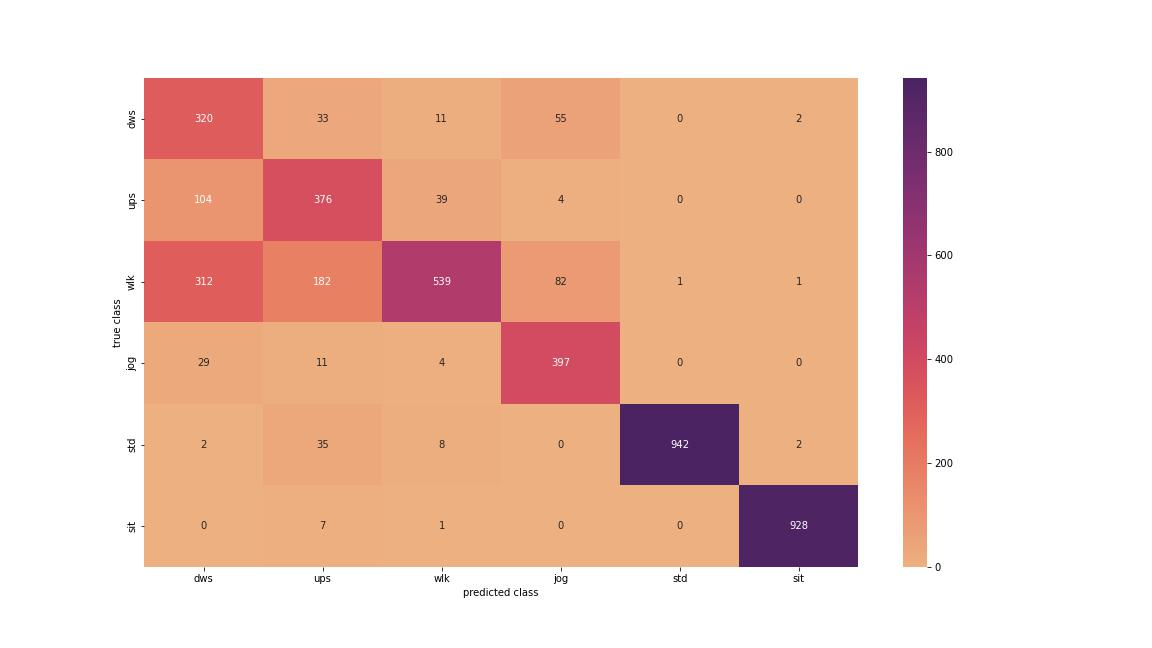
\includegraphics[width=\linewidth]{conf_mat_mos.jpg}
	\caption[Confusion matrix MotionSense]{Confusion matrix of MAF + Bayes classifier on MotionSense data, settings of MAF are W=True, T=64, A=True, N=True (own image).}
	\label{fig:confm}
\end{figure}

\begin{figure}
	\centering
	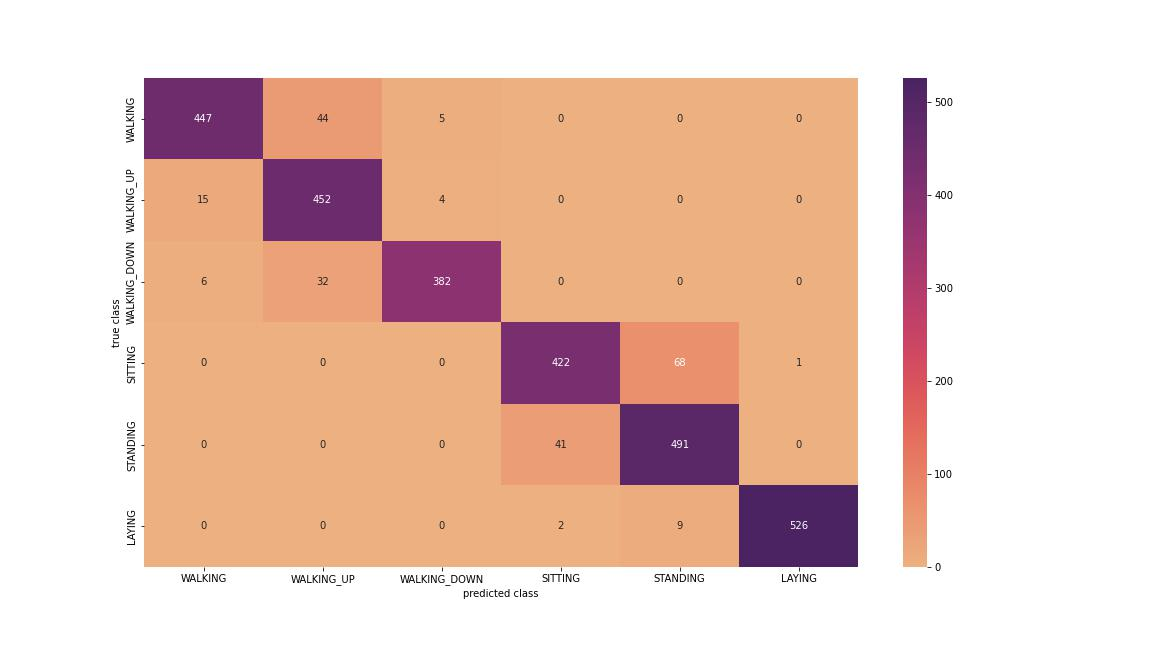
\includegraphics[width=\linewidth]{conf_mat_uci.jpg}
	\caption[Confusion matrix UCIHAR]{Confusion matrix of MAF + Bayes classifier on UCI HAR data, settings of MAF are W=True, T=128, A=False, N=False (own image).}
	\label{fig:confu}
\end{figure}

\begin{figure}
	\centering
	\includegraphics[width=\linewidth]{pairplot.png}
	\caption[Pairplot Carrot]{Pairplot of Carrot dataset features, the histograms on the main diagonal show the distribution of each feature (own image).}
	\label{fig:pair}
\end{figure}


\newpage


\pagestyle{empty}


\section*{Ehrenw\"ortliche Erkl\"arung}
Ich versichere, dass ich die beiliegende Master-/Bachelorarbeit ohne Hilfe Dritter
und ohne Benutzung anderer als der angegebenen Quellen und Hilfsmittel
angefertigt und die den benutzten Quellen w\"ortlich oder inhaltlich
entnommenen Stellen als solche kenntlich gemacht habe. Diese Arbeit
hat in gleicher oder \"ahnlicher Form noch keiner Pr\"ufungsbeh\"orde
vorgelegen. Ich bin mir bewusst, dass eine falsche Erkl\"arung rechtliche Folgen haben
wird.
\\
\\

\noindent
Mannheim, den 15.01.2023 \hspace{4cm} Unterschrift

\end{document}
